\chapter{Physics-based Lidar Simulation - Propagation or radiometry}
\section{Experimental Setup}
The propagation mode is valuated by the prototype lidar by measuring the peak power of signals reflected by targets at different distance. An oscilloscope is used for the signal acquisition, and five signals were collected for each distance. The experimental setup is given in Figure \todo{add setup figure}. The parameters utilized in the propagation model is given in Table \todo{add parameter table}
\section{Validation Result}
The measured peak power and the corresponding result modeled by the propagation model is given in Figure~\ref{fig:prop_valid}, from which we can see the result from the propagation model and the oscilloscope measurement mainly follows the same trend. The difference could be due to the usage of aluminum foils, since the reflected energy may vary when the target was moved from one position to another one.
\begin{figure}[t!p]
\centering
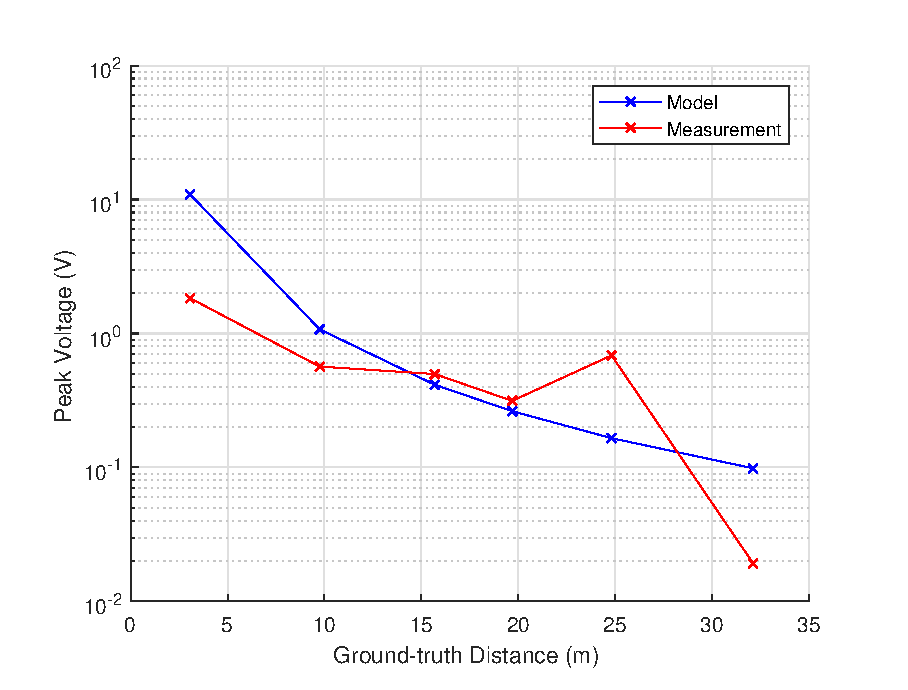
\includegraphics[width=1\textwidth]{figures/chapter_propagation/Res_validation_Vp_distance.eps}
\caption{Peak power of modeled signal and oscilloscope measurements}
\label{fig:prop_valid}
\end{figure}
